\documentclass[../main.tex]{subfiles}
\begin{document}

\chapter{Überblick}
\label{overview}
\pagenumbering{arabic}
  Virtualisierung entwickelte sich in den letzten Jahren zu einem allgegenwärtigen Thema in der Informatik. Mehrere Virtualisierungstypen entstanden, als von akademische und industrielle Forschungsgruppen vielseitige Einsatzmöglichkeiten der Virtualisierung aufgedeckt wurden.

  Allgemein versteht man unter ihr die Nachahmung und Abstraktion von physischen Resourcen, z.B. der \acrshort{CPU} oder des Speichers, die in einem virtuellen Kontext von Softwareprogrammen genutzt wird.

  Die Vorteile von Virtualisierung umfassen Hardwareunabhängigkeit, Verfügbarkeit, Isolierung und Sicherheit, welche die Erfolgsgrundlage der Virtualisierung in heutigen \gls{Cloud}-Infrastrukturen bilden \cite[S.1]{containerVirtPerformance}. Vor allem in Rechenzentren bieten sich Virtualisierungen an, um die Serverressourcen effizienter zu nutzen \cite[S.1]{dockerSec1}. Letztendlich haben es Virtualisierungen ermöglicht, Serverressourcen in der Form von \glspl{Cloud}, wie z.B. den \emph{Amazon Web Services}\cite{amazonWebServices}, und auf Basis eines Subskriptionsmodells nutzen zu können \cite[S.1]{dockerSec1}.

  Heutzutage existieren mehrere serverseitige Virtualisierungstechniken, wovon die Hypervisor-gestützen Methoden mit den etablierten Vertretern \emph{Xen}\cite{xen}, \emph{KVM}\cite{kvm}, \emph{VMware ESXi}\cite{vmwareESXi} und \emph{Hyper-V}\cite{hyperv} die meistverbreitesten sind \cite[S.2]{containerVirtPerformance}. Die alternative containerbasierte Virtualisierung, auch Virtualisierung auf Betriebssystemebene (\emph{Operating System-Level Virtualization}) genannt, wurde in den letzten Jahren durch ihre leichtgewichtige Natur zunehmend beliebt und erlebte mit dem Erfolg von Docker, seit dessen Release im März 2013, einen medienwirksamen Aufschwung \cite{githubDockerChangelog}. Wie die \emph{Google Trends} in \fig \ref{fig:overview_googleTrends} zeigen, stieg das Interesse an Docker seit dessen Release kontinuierlich an, während das Suchwort \glqq{}virtualization\grqq{} im Jahr 2010 seinen Höhepunkt hatte und seitdem an Popularität verlor. Auch das Interesse an der Containertechnologie \emph{LXC}, aus der Docker entstand, bleibt weit hinter der von Docker zurück \cite{googleTrends}.

  \begin{figure}[h]
      \centering
      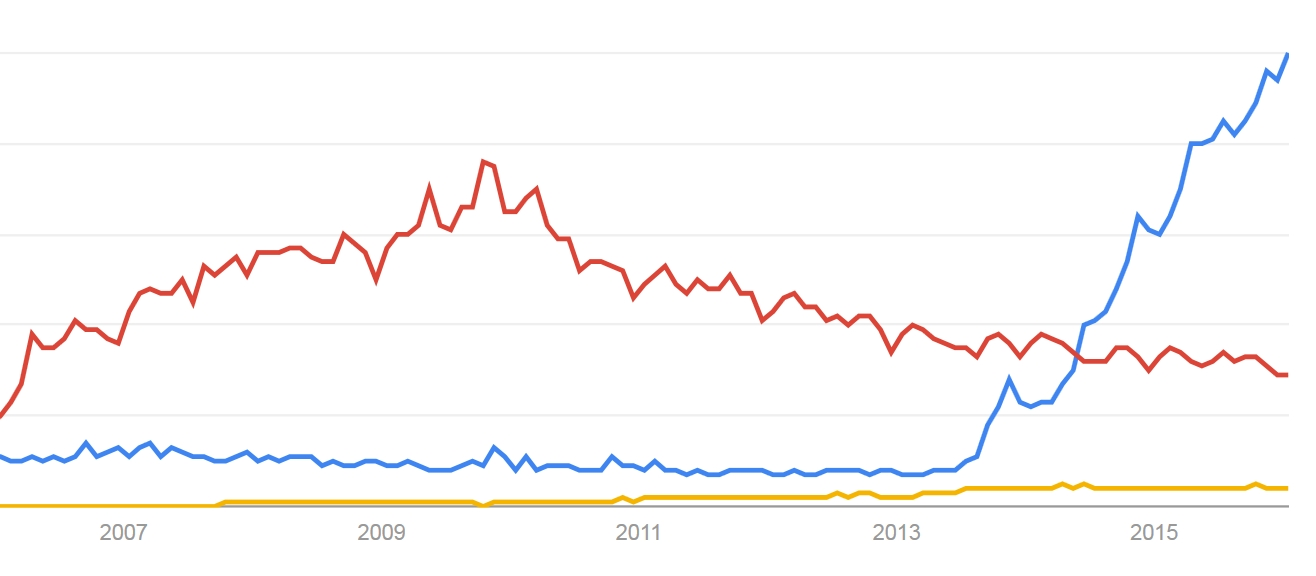
\includegraphics[width=1.0\textwidth]{./images/googletrend_dockerVirtualizationLXC.jpg}
      \caption{Google Trends der Suchbegriffe \glqq{}Virtualization\grqq{} (rot), \glqq{}Docker\grqq{} (blau) und \glqq{}LXC\grqq{} (gelb) von Januar 2006 bis Januar 2016\cite{googleTrends}.}
      \label{fig:overview_googleTrends}
  \end{figure}

  Obwohl das Konzept von Containern bereits im Jahr 2000 als \emph{Jails} in dem Betriebssystem \emph{FreeBSD} und seit 2004 als \emph{Zones} unter \emph{Solaris} verwendet wurde \cite{zonesReleasenotes}\cite{jailsReleasenotes}, gelang keiner dieser Technologien vor Docker der Durchbruch. Wie Docker den bis 2013 vorherrschenden Ruf von Containertechnologien, dass Container noch nicht ausgereift seien \cite[S.8]{containerVirtPerformance}, nachhaltig verändern konnte, ist in der Einführung zu Docker in Kapitel \ref{dockerIntro} beschreiben.

  Heute sind Container in vielen Szenarien, v.a. skalierbaren Infrastrukturen, trotz intrinsischer Sicherheitsdefizite gegenüber Hypervisor-gestützten Virtualisierungsarten beliebt. Vor allem \glspl{MultiTenantService} werden gerne mit Docker umgesetzt \cite[S.6]{dockerBook}\cite{dockerUnderstandingDocker}.

  % TODO: (eigene Worte --> Evtl als Einleitung fuer FORSCHUNGSFRAGE,PROBLEM)
  % Vor der Virtualisierung waren Hosts physisch getrennt, sprich auf unterschiedlichen physischen Maschinen. Angriffe waren nur über das Netzwerk möglich, die einzigste Komponente, die Hosts verbindet.
  % Mit der Virtualisierung exisitiert weiterhin die Gefahr über das Netzwerk, jedoch kommt eine weitere Komponente hinzu: die Systemsicherheit. Da sich, unabhängig von der eingesetzten Virtualisierungstechnik, mehrere Gastsysteme einen physischen Host teilen, können Angriffe auch innerhalb eines physischen Hosts ablaufen und diesen oder andere virtuelle Gastinstanzen zum Ziel haben. Angriffe nutzen bekannte und nicht behobene, oder unbekannte (sogenannte \emph{Zero-Day-Exploits}) Sicherheitslücken von Kernel- oder Anwendungsprogrammen, um ihr Ziel zu erreichen.


  % https://www.airpair.com/firebase/posts/yatodo-guide
  % https://www.airpair.com/docker/posts/8-proven-real-world-ways-to-use-docker#7-multi-tenancy

  % TODO: Oft in Github-Repos geforscht, da offizielle Docker Docs teilweise hinterherhinken. Aktuelle Diskussionen sind in github issues mit drin, da dort auch problem eroertert werden. In den docker-docs und docker-blogeintraegen oft nur "wow docker kann jetyzt auch das"

  \section{Ziel der Arbeit}
    Ziel der Arbeit ist es, die von Containersystemen genutzten Sicherheitsmechanismen vorzustellen und zu untersuchen, inwiefern diese zu im Fall von Docker zu einer höheren Sicherheit des Systems beitragen.

    Eine ausführliche Konstruktion der Fragestellung erfolgt mithilfe einer Risikoanalyse in Kapitel \ref{question}.

  \section{Struktur der Arbeit}
    Zu Beginn wird in den Grundlagen ab Kapitel \ref{introVirt} die Virtualisierung beschrieben. Dabei werden die zwei prominentesten Virtualisierungstechniken, Hypervisor-basierte (Sektion \ref{introVirtHypervisor}) und Container-basierte (Sektion \ref{introVirtContainer}) Virtualisierung, gegenübergestellt. In diesem Kapitel werden nur die für diese Arbeit relevante Techniken der Systemvirtualisierung beschrieben, also solche, in denen Funktionen von kompletten Betriebssystemen abstrahiert werden. Andere Arten, beispielsweise die Anwendungs-, Storage- oder Netzwerkvirtualisierung, werden nicht behandelt, da sie isoliert keinen Bezug zu Docker haben. Anschließend werden die allgemeinen Sicherheitsziele von \acrshort{IT}-Systemen in Kapitel \ref{introSecGoals} erklärt, auf die im Hauptteil Bezug genommen wird. Abgeschlossen wird das Grundlagenkapitel mit einer Einführung in Docker (Kapitel \ref{dockerIntro}), in dem Begriffe sowie Funktionsweisen innerhalb dieser Technologie erläutert werden.

    Die genannten Grundlagen sind sehr weitreichende Themengebiete. Um in den einleitenden Kapiteln nicht ausführlich zu werden, sind Eckdaten einiger am Rande auftretender Begriffe im angehängten Glossar zusammengefasst.

    Der Hauptteil ab Kapitel \ref{secLinux} untergliedert sich in mehrere Sicherheitsgebiete, in die die Arbeit eingeteilt ist:
    \begin{enumerate}
      \item \textbf{Sicherheitsmechanismen, die Linux ermöglicht} und teils obligatorisch von Docker eingesetzt werden. Darunter fallen Techniken zur Isolierung, Ressourcen- und Rechteverwaltung von Containern sowie Methoden, um das Hostsystem mit zusätzlichen Sicherheitsfeatures von Linux abzusichern.
      \item \textbf{Sicherheit im Docker-Ökosystem}. Darunter fallen z.B.
        \begin{itemize}
          \item Integrität von Images
          \item Absicherung der Kommunikation zwischen dem Docker-Client und dem Docker-Host
          \item \glspl{BestPractice} im Umgang mit Docker-Komponenten sowie Sicherheitsrichtlinien.
          \item Verwendung von Third-Party Tools, wie \emph{Kubernetes} % TODO: Glossareintrag Third-Party
        \end{itemize}
      \item \textbf{Sicherheit von Docker in Cloud-Infrastrukturen}. Gegenstand der Untersuchung ist, ob und wie Docker in der Cloud eingesetzt werden kann, sodass Sicherheitsanforderungen von Unternehmen erfüllt werden.
        % TODO: Etwas mehr Details dazu, wenn klar ist was hier reinkommt.
    \end{enumerate}

    Abgeschlossen wird die Arbeit im letzten Kapitel \ref{result} mit einer Zusammenfassung der Erkenntnisse und einem Ausblick auf die Zukunft von Docker und der containerbasierten Virtualisierung.

    In der Arbeit vorkommende Produkt-, Technologie-, Bibliotheken- und Unternehmensnamen sind durchgehend \emph{kursiv} gedruckt. Eine Ausnahme bildet Docker, in der die reguläre Schreibweise für die Plattform Docker vorgesehen ist, während die kursive Variante das Unternehmen \emph{Docker} meint.

    Im Gegensatz dazu sind technische Identifikationsmerkmale, Befehle und Variablennamen \texttt{mono-type} geschrieben. Platzhalter für aufgeführte Befehlsparameter sind in Großbuchstaben abgedruckt. Ein Befehl \texttt{cmd} beispielsweise, der einen Parameter erwartet, ist dementsprechend als \texttt{cmd PARAMETER} generisch formuliert.
\end{document}
